\section{Use Cases}

A use case is a~term that describes how actors use a~program to achieve specific goals.
They describe and organize functional requirements from the~end users' point of view.
They are sequences of events and interactions that users can easily follow to achieve specific goals.
Use cases have primary and can optionally have secondary scenarios of their flow.

Each use case has a~name, triggering events, and the~main flow of events.
The~name contains a~verb and a~noun that express the~goal of the~use case.
The~triggering events describe an~initiation of the~use case.
Each use case can have multiple triggering events.
And the~main flow of events, step by step, describes the~flow of interactions between the~system and the~actor.
Optionally, use cases can also have preconditions.
Preconditions are conditions that must be met before executing the~use case.
Initiation and preconditions are a~part of the~flow, but they can be described separately.

Use cases of designed game recognize two actors: an~Anonymous User, an~actor who is not signed in to the~game, and a~Player, an~actor who is signed in to the~game.
The~Player is an~extension of the~Anonymous User.
That means that the~Player can use or execute everything the~Anonymous User can use or execute.

\let\oldsubsection=\thesubsection
\renewcommand\thesubsection{UC\arabic{subsection}}

\pagebreak
\subsection{Sign Up}

This use case describes signing up for the~game and is used by an~Anonymous User who, if processed successfully, becomes a~Player actor. If a~Player actor tries to activate the~use case, they are redirected to the~main screen.

This use case starts when an~actor navigates to the~sign-up screen or activates the~sign-up button.

\begin{enumerate}
    \item The~game navigates the~actor to the~sign-up screen.
    \item The~actor fills in their username, real name, email, password, and\linebreak{}description into text inputs.
    \item The~game determines the~validity of the~actor's data.
    \begin{enumerate}
        \item If no issues were found, the~game signs in the~actor and navigates them to their profile screen.
        the~actor becomes a~Player.
        \item If issues were found, the~game announces the~fail.
    \end{enumerate}
\end{enumerate}

\subsection{Sign In}

This use case describes the~signing in the~game, and only an~Anonymous User can use it. If a~Player actor tries to activate the~use case, they are redirected to the~main screen.
If processed successfully, the~actor becomes a~Player actor.

This use case starts when an~actor navigates to the~sign-in screen or activates the~sign-in button.

\begin{enumerate}
    \item The~game navigates the~actor to the~sign-in screen.
    \item The~actor fills in their username and password into text inputs.
    \item The~game determines the~validity of provided username and the~corresponding password.
    \begin{enumerate}
        \item If no issues were found, the~game signs in the~actor and navigates them to their profile screen. The~actor becomes a~Player.
        \item If issues were found, the~game announces the~fail.
    \end{enumerate}
\end{enumerate}

\subsection{Sign Out}

This use case describes signing out of the~game, and only a~Player actor can use it.
After processing the~use case, the~actor becomes an~Anonymous User.

This use case starts when an~actor activates the~sign-out button.

\begin{enumerate}
    \item The~game signs the~actor out of the~game.
    \item The~actor is navigated to the~main screen.
\end{enumerate}

\subsection{View Publicly Available Game Information}

This use case describes viewing the~publicly available game information and other publicly available screens like the~main screen and about-us screen and its subscreens.
It can be used by an~Anonymous User actor, which also extends the~use to the~Player actor.

This use case starts when an~actor navigates to the~main screen, \mbox{about-us} screen, or its subscreens, activates the~main-screen button, or navigates to or activates any other screen or buttons, leading to screens with publicly available information.

\subsubsection*{Scenario A~--- Main Screen}

\begin{enumerate}
    \item The~game navigates the~actor to the~main screen.
    \item There, the~actor can view the~information.
\end{enumerate}

\subsubsection*{Scenario B~--- About-Us Screen}

\begin{enumerate}
    \item The~game navigates the~actor to the~about-us screen (or one of its \mbox{corresponding} subscreens).
    \item There, the~actor can view the~information.
\end{enumerate}

\subsection{View Own Profile}

This use case describes viewing an~actor's in-game profile.
A Player actor can only use it.
If an~actor, not a~Player, tries to activate the~use case, they are redirected to the~sign-in screen.

This use case starts when an~actor navigates to the~profile screen or activates the~profile button.

\begin{enumerate}
    \item The~game navigates them to their profile screen.
    \item There, the~actor can view the~profile.
\end{enumerate}

\subsection{View Own Statistics}

This use case describes viewing an~actor's in-game statistics.
A Player actor can only use it.
If an~actor, not a~Player, tries to activate the~use case, they are redirected to the~sign-in screen.

This use case starts when an~actor navigates to the~statistics screen or activates the~profile button.

\begin{enumerate}
    \item The~game navigates the~user to their statistics screen.
    \item There, the~actor can view the~statistics.
\end{enumerate}

\pagebreak
\subsection{View Courses}

This use case describes viewing a~list of game courses~--- called stories~--- a~specific story, and a~list of the~story's missions.
A Player actor can only use it.
If an~actor, not a~Player, tries to activate the~use case, they are redirected to the~sign-in screen.

This use case starts differently based on its scenarios.

\subsubsection*{Scenario A~--- View Courses}

This scenario starts when an~actor navigates to the~stories screen or activates the~stories button.

\begin{enumerate}
    \item The~game navigates the~actor to the~stories screen.
    \item The~actor can view a~list of courses.
\end{enumerate}

\subsubsection*{Scenario B~--- View Course}

This scenario starts when an~actor navigates to the~story screen or activates the~specific story button.

\begin{enumerate}
    \item The~game navigates the~actor to the~selected story screen.
    \item The~actor can view a~list of the~story's missions and the~story's name and description.
\end{enumerate}

\subsubsection*{Scenario C~--- View Mission}

This scenario starts when, on the~story screen, an~actor activates the~mission's item or button.

\begin{enumerate}
    \item The~game displays a~popup containing additional data about the~mission.
    It displays the~mission's name and description.
    \item If it is a~storytelling mission, a~\textquote*{read} button is displayed.
    \item If it is a~learning mission, a~\textquote*{learn} button is displayed.
    \item If it is a~game mission, a~\textquote*{play} button is displayed.
    \item The~actor can activate the~displayed button to leave the~screen.
\end{enumerate}

\pagebreak
\subsection{Use Missions}

This use case describes using and viewing the~game mission.
A Player actor can only use it.
If an~actor, not a~Player, tries to activate the~use case, they are redirected to the~sign-in screen.

This use case starts when an~actor navigates to the~story's mission screen or activates the~mission's item or button on the~story screen.

\subsubsection*{Scenario A~--- Storytelling Mission}

This scenario starts when an~actor navigates to the~storytelling mission or activates the~storytelling mission's item or button on the~story screen.

\begin{enumerate}
    \item The~game navigates the~actor to the~storytelling mission screen.
    \item The~actor is presented with a~list of texts that can be shown step by step by clicking the~next button.
    \item The~\textquote*{Back to story} button is displayed after the~actor progresses through all the~texts.
    \item Using the~\textquote*{Back to story} button, the~actor can leave the~screen to the~mission's story screen.
\end{enumerate}

\subsubsection*{Scenario B~--- Learning Mission}

This scenario starts when an~actor navigates to the~learning mission or activates the~learning mission's item or button on the~story screen.

\begin{enumerate}
    \item The~game navigates the~actor to the~learning mission screen.
    \item The~actor is presented with a~learning text.
    \item The~\textquote*{Back to story} button is displayed.
    \item Using the~\textquote*{Back to story} button, the~actor can leave the~screen to the~mission's story screen.
\end{enumerate}

\subsubsection*{Scenario C~--- Game Mission}

This scenario starts when an~actor navigates to the~game mission or activates the~game mission's item or button on the~story screen.

\begin{enumerate}
    \item The~game navigates the~actor to the~game mission screen.
    \item The~actor is presented with a~game grid, command list view, and buttons that control the~mission.
    \item The~user can add or move commands, run or stop the~current game or save the~current game~--- as described in custom use cases.
\end{enumerate}

\subsection{Save Current Game}

This use case describes the~saving of the~actor's current game.
A Player actor can only use it.

This use case starts when an~actor activates the~save button on the~game mission screen.
Being on the~game mission screen is a~precondition of this use case.

\begin{enumerate}
    \item The~game loads the~current progress of the~commands presented in the~command list view.
    \item The~game saves those data, together with completed, size, and speed attributes. 
\end{enumerate}

\subsection{Play Current Game}

This use case describes the~playing of the~actor's current game.
A Player actor can only use it.

This use case starts when an~actor activates the~play button on the~game mission screen.
Being on the~game mission screen is a~precondition of this use case.

\begin{enumerate}
    \item The~game locks the~command list view, so the~actor cannot interact with it. 
    \item The~game loads the~current progress of the~commands presented in the~command list view.
    \item The~game process these commands.
    \item The~game starts presenting a~step-by-step progression of the~game grid.
    the~procession of each step is signalized by an~arrow next to a~command block.
    \item After a~presentation is done, the~game shows a~dialog with optional size and speed challenge attributes.
    \begin{enumerate}
        \item If the~game resulted in a~success, a~success dialog is presented with a~corresponding status message.
        \item If the~game resulted in a~failure, a~failure dialog is presented with a~corresponding status message and related error message.
    \end{enumerate}
    \item The~game unlocks the~command list view.
    \item The~game saves the~current progression, as described in the~separate use case. 
\end{enumerate}

\subsection{Stop Current Game}

This use case describes the~stopping of the~actor's current game.
A Player actor can only use it.

This use case starts when an~actor activates the~stop button on the~game mission screen while the~game is in progress.
Being on the~game mission screen with a~game in progress is a~precondition of this use case.

\begin{enumerate}
    \item The~game stops the~progressing game.
    \item The~game unlocks the~command list view.
    \item The~game does not save the~progression and does not show the~success or failure dialog. 
\end{enumerate}

\let\thesubsection=\oldsubsection

\subsection{Requirements Implementation Overview}

\begin{table}[b]
    \catcode`\-=12
    \centering
    \begin{tabular}{lcccccccc}
    \toprule
    & \multicolumn{8}{c}{Functional Requirements} \\
    \cmidrule(l){2-9}
    Use Case & F1 & F2 & F3 & F4 & F5 & F6 & F7 & F8  \\
    \midrule
                         UC1  & $\ast$ &        &        &        &        &        &        &         \\
    \rowcolor[gray]{.95} UC2  & $\ast$ &        &        &        &        &        &        &         \\
                         UC3  & $\ast$ &        &        &        &        &        &        &         \\
    \rowcolor[gray]{.95} UC4  &        & $\ast$ &        &        &        &        &        &         \\
                         UC5  &        &        &        & $\ast$ &        &        &        &         \\
    \rowcolor[gray]{.95} UC6  &        &        & $\ast$ &        &        &        &        &         \\
                         UC7  &        &        &        &        & $\ast$ & $\ast$ & $\ast$ & $\ast$  \\
    \rowcolor[gray]{.95} UC8  &        &        &        &        &        & $\ast$ & $\ast$ & $\ast$  \\
                         UC9  &        &        &        &        &        &        &        & $\ast$  \\
    \rowcolor[gray]{.95} UC10 &        &        &        &        &        &        &        & $\ast$  \\
                         UC11 &        &        &        &        &        &        &        & $\ast$  \\
    \bottomrule
    \end{tabular}
    \caption{Implementation of Use Cases and Compliance with Requirements}
    \label{table:usecases-requirements}
\end{table}

Use cases organize functional requirements. 
An overview of the~implementation of use cases by functional requirements can be seen in the table~\ref{table:usecases-requirements}.

Use cases distinguish two actors, an~Anonymous User and a~Player.
\linebreak
The~Player actor is an~extension of the~Anonymous User actor.
The~competence of both actors and relationships of individual use cases can be seen in the~figure~\ref{fig:usecasediagram}.

\begin{figure}
    \centering
    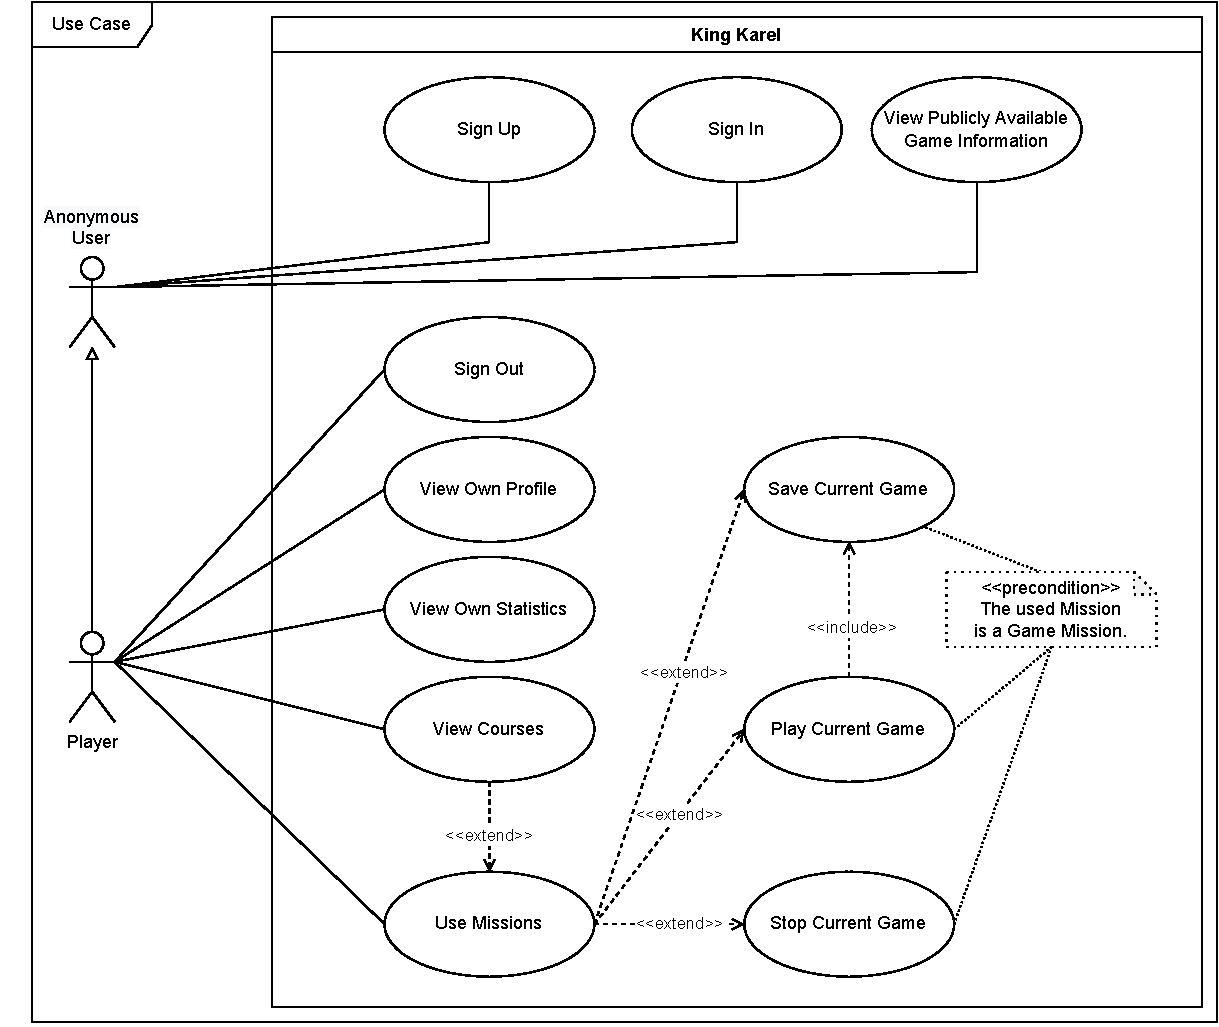
\includegraphics[width=1\linewidth]{assets/design/usecasediagram.pdf}
    \caption{Use Case Diagram}
    \label{fig:usecasediagram}
\end{figure}
